%\title{LaTeX Portrait Poster Template}
%%%%%%%%%%%%%%%%%%%%%%%%%%%%%%%%%%%%%%%%%
% a0poster Portrait Poster
% LaTeX Template
% Version 1.0 (22/06/13)
%
% The a0poster class was created by:
% Gerlinde Kettl and Matthias Weiser (tex@kettl.de)
% 
% Adapter by Jens Buysse for Hogeschool Gent
% This template has been downloaded from:
% http://www.LaTeXTemplates.com
%
% License:
% CC BY-NC-SA 3.0 (http://creativecommons.org/licenses/by-nc-sa/3.0/)
%
%%%%%%%%%%%%%%%%%%%%%%%%%%%%%%%%%%%%%%%%%

%----------------------------------------------------------------------------------------
%	PACKAGES AND OTHER DOCUMENT CONFIGURATIONS
%----------------------------------------------------------------------------------------

\documentclass[a0,portrait]{a0poster}

\usepackage{multicol} % This is so we can have multiple columns of text side-by-side
\columnsep=100pt % This is the amount of white space between the columns in the poster
\columnseprule=3pt % This is the thickness of the black line between the columns in the poster

\usepackage[svgnames]{xcolor} % Specify colors by their 'svgnames', for a full list of all colors available see here: http://www.latextemplates.com/svgnames-colors

\usepackage{times} % Use the times font
%\usepackage{palatino} % Uncomment to use the Palatino font

\usepackage{graphicx} % Required for including images
\graphicspath{{figures/}} % Location of the graphics files
\usepackage{booktabs} % Top and bottom rules for table
\usepackage[font=small,labelfont=bf]{caption} % Required for specifying captions to tables and figures
\usepackage{amsfonts, amsmath, amsthm, amssymb} % For math fonts, symbols and environments
\usepackage{wrapfig} % Allows wrapping text around tables and figures
\usepackage[export]{adjustbox}
\usepackage{caption}

\begin{document}

%----------------------------------------------------------------------------------------
%	POSTER HEADER 
%----------------------------------------------------------------------------------------

% The header is divided into two boxes:
% The first is 75% wide and houses the title, subtitle, names, university/organization and contact information
% The second is 25% wide and houses a logo for your university/organization or a photo of you
% The widths of these boxes can be easily edited to accommodate your content as you see fit

\begin{minipage}[t]{0.75\linewidth}
\VeryHuge \color{HoGentAccent1} \textbf{Kotlin/Native, het nieuwe cross-platform framework voor de mobiele omgeving} \color{Black}\\ % Title
%\Huge\textit{Ondertitel (eventueel)}\\[2.4cm] % Subtitle
\huge \textbf{Van Wassenhove Ilias, Goossens Sander, Van Schoor Johan}\\[0.5cm] % Author(s)
\huge Hogeschool Gent, Valentin Vaerwyckweg 1, 9000 Gent\\[0.4cm] % University/organization
\Large \texttt{ilias.vanwassenhove.w9579@student.hogent.be} \\
\end{minipage}
%
\begin{minipage}[t]{0.25\linewidth}

\includegraphics[width=13cm,right]{figures/HG-woordmerk.jpg} 

\end{minipage}

\vspace{1cm} % A bit of extra whitespace between the header and poster content

%----------------------------------------------------------------------------------------

\begin{multicols}{2} % This is how many columns your poster will be broken into, a portrait poster is generally split into 2 columns

%----------------------------------------------------------------------------------------
%	ABSTRACT
%----------------------------------------------------------------------------------------

\color{HoGentAccent1} % Navy color for the abstract

\begin{abstract}
Nog niet zo lang geleden had men bij het bouwen van mobiele applicaties (Android, iOS en Windows) enkel en alleen de mogelijkheid om drie aparte applicaties te bouwen, namelijk native applicaties. Dit vergde veel werk en was heel kostelijk voor veel bedrijven. Enerzijds is er per platform de tijd en kost om de applicatie te ontwikkelen, anderzijds is er de kost om deze applicaties uit te breiden of te onderhouden. Als reactie hierop zijn de cross-platform frameworks uitgevonden, denk maar aan: React, Xamarin en Ionic met Angular. Bij deze frameworks moet er maar éénmalig code geschreven worden, de user interface is hetzelfde voor alle platformen en het framework zorgt ervoor dat de applicatie op elk besturingssysteem kan draaien. Een kleine nuance, origineel had Xamarin niet de mogelijkheid om één user interface te ontwikkelen die hetzelfde was voor alle platformen. Er mag misschien nog een framework toegevoegd worden aan het lijstje van frameworks om cross-platform applicaties te ontwikkelen, namelijk Kotlin/Native.

\begin{center}\vspace{1cm}
	
\includegraphics[width=1.0\linewidth]{figures/kotlin.png}
	\captionof{figure}{\color{HoGentAccent5}Kotlin logo}
\end{center}\vspace{1cm}

\end{abstract}
%----------------------------------------------------------------------------------------
%	INTRODUCTION
%----------------------------------------------------------------------------------------

\color{HoGentAccent1} 
\section*{Introductie}
\color{black}
\color{black}
Kotlin is een nieuwe programmeertaal die geintroduceerd werd in 2011 door JetBrains. JetBrains is een organisatie afkomstig van Sint- Petersburg, Rusland. De naam Kotlin is afkomstig van het Kotlin eiland, 30 km ten westen van Sint-Petersburg. JetBrains is een software ontwikkelingbedrijf dat gesticht is in het jaar 2000. Hun hoofdkantoor is gevestigd in Praag (Tsjechië) en hun core-business is het ontwikkelen van tools die gebruikt kunnen worden door verschillende types van software ontwikkelaars. Zo hebben zij IDE’s ontwikkeld voor Java, Ruby, Python, PHP, SQL, Objective-C, C++, C\# en JavaScript.
\newline
\newline
Origineel is het een programmeertaal die draait op de Java Virtual Machine (JVM). Maar JetBrains is veel verder gegaan dan toestellen die een JVM kunnen draaien. Met Kotlin/Native hebben ze zich gericht tot alle platformen en besturingssystemen. In dit onderzoek zal onderzocht hoe JetBrains ervoor gezorgd heeft dat Kotlin code op ieder platform kan worden gebruikt. Kotlin/Native maakt gebruik van de LLVM compiler en hierdoor zal de werking van deze compiler bestudeerd worden. Daarnaast werd onderzocht hoe Kotlin/Native werkt en hoe het gebruikt kan worden voor cross-platform applicatieontwikkeling.

\begin{center}\vspace{1cm}
	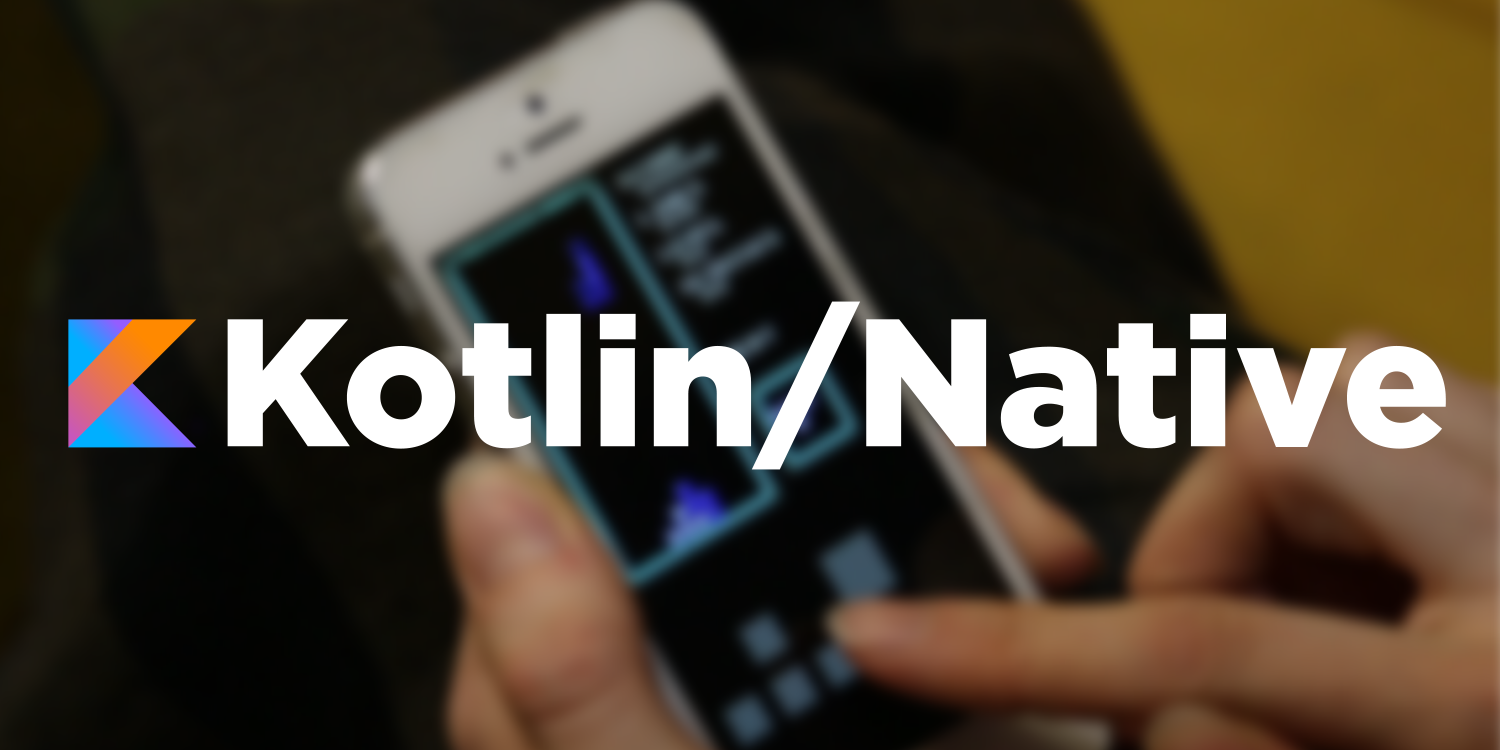
\includegraphics[width=1.0\linewidth]{figures/kn.png}
	\captionof{figure}{\color{HoGentAccent5}Kotlin/Native voor cross-platform applicatieontwikkeling}
\end{center}\vspace{1cm}
%----------------------------------------------------------------------------------------
%	GEOLOGY
%----------------------------------------------------------------------------------------

\color{Black} % DarkSlateGray color for the rest of the content
\color{HoGentAccent1} 
\section*{Experimenten}
\color{black}
Voor dit onderzoek werd er praktisch aan de slag gegaan met Kotlin/Native. Eerst en vooral werden de voorbeeldprojecten van JetBrains onderzocht. Hierdoor werd de opzet van een Kotlin/Native project duidelijk. Daarnaast werd de Kotlin/Native plugin bekeken speciaal voor iOS development. Eens de werking van Kotlin/Native duidelijk was, werd er een kleine shopping-applicatie gemaakt dat zowel Android als iOS ondersteunt. De gebruiker kan op deze applicatie een winkelmandje aanmaken, alle producten bekijken en eventueel de details van een product opvragen. Hij heeft ook de mogelijkheid om een product toe te voegen aan zijn winkelmandje en om zijn winkelmandje te bekijken. Door gebruik te maken van Kotlin/Native wordt alle domeinlogica van deze applicatie gedeeld over de verschillende ondersteunde platformen, dit zijnde iOS en Android.

\begin{center}\vspace{1cm}
	
\includegraphics[width=1.0\linewidth]{figures/apple-android.jpeg}
	\captionof{figure}{\color{HoGentAccent5}Ondersteunde platformen van de proof-of-concept}
\end{center}\vspace{1cm}

\iffalse
\color{HoGentAccent1} 
\section*{Sectie met figuur}
\color{black}


\begin{center}\vspace{1cm}

\includegraphics[width=1.0\linewidth]{grail}
\captionof{figure}{\color{HoGentAccent5} He hasn't got shit all over him. The nose? Where'd you get the coconuts? What do you mean? We shall say 'Ni' again to you, if you do not appease us}
\end{center}\vspace{1cm}
\fi

%------------------------------------------------



\color{HoGentAccent1} 
\section*{Conclusies}
\color{black}
Kotlin/Native beschikt reeds over de capaciteiten om gebruikt te worden als een cross-platform framework. Echter zijn de mogelijkheden nog beperkt. Het framework is nog zeer jong en de huidige versie is slechts 0.6. Er is duidelijk eerst en vooral nood aan een stabiele versie waarmee ontwikkelaars aan de slag kunnen. Indien een applicatie over een grote en ingewikkelde domeinlogica beschikt, heeft dit framework zeker en vast een groot voordeel ten opzichte van native Android- en iOS-applicaties. Echter moet de user interface per platform worden opgebouwd. Er is nog geen mogelijkheid om via Kotlin/Native een user interface op te bouwen. Dit kan zowel positief als negatief beschouwd worden. Enerzijds is er de mogelijkheid om verschillen aan te brengen in de user interface per platform, anderzijds moeten er dus verschillende interfaces gebouwd worden wat dubbel zoveel tijd en geld kost om te ontwikkelen. Het is dus reeds mogelijk om aan de slag te gaan met dit framework, echter is het niet gemakkelijk. Dit aangezien er momenteel geen plugin bestaat om te installeren in een IDE zoals IntelliJ en er is geen officiële documentatie beschikbaar over de opzet van een Kotlin/Native project. Maar aan de hand van de proof-of-concept kan besloten worden dat Kotlin/Native momenteel wel reeds kan worden gebruikt om domeinlogica te delen over verschillende platformen. Het is dus mogelijk om domeinlogica, die geschreven is in Kotlin, te gebruiken voor iOS.
%----------------------------------------------------------------------------------------
%	FORTHCOMING RESEARCH
%----------------------------------------------------------------------------------------
\color{HoGentAccent1} 
\section*{Toekomstig onderzoek}
\color{black}
Wat toekomstig onderzoek betreft in verband met Kotlin/Native is er nog veel mogelijk. Er kan onderzocht worden of er de mogelijkheid is om een plugin te ontwikkelen voor een IDE waardoor de opzet van een project mogelijk zou zijn via enkele klikken. Verder kan eventueel bekeken worden hoe men in de Kotlin code gebruik kan maken van iOS protocollen en andere bibliotheken. Ten slotte is het aanspreken van hardware, zoals de camera, totaal nog niet onderzocht voor Kotlin/Native. Zoals te lezen is, is er nog veel ruimte tot onderzoek voor dit framework.

\begin{center}\vspace{1cm}
	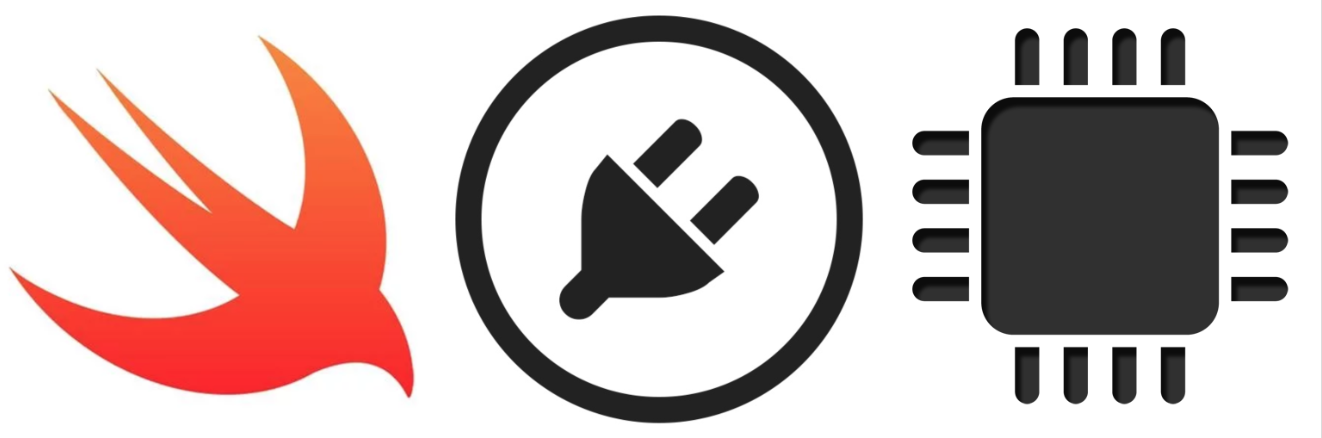
\includegraphics[width=1.0\linewidth]{figures/verder-onderzoek.png}
	\captionof{figure}{\color{HoGentAccent5}Swift logo, plugin en hardware icon}
\end{center}\vspace{1cm}

%----------------------------------------------------------------------------------------

\end{multicols}
\end{document}